% Chapter Template

\chapter{Theory} % Main chapter title
\label{Theory} % Change X to a consecutive number; for referencing this chapter elsewhere, use \ref{ChapterX}

\lhead{Chapter \ref{Theory}. \emph{Theory}} % Change X to a consecutive number; this is for the header on each page - perhaps a shortened title

\section{Ontology and folksonomy}
One of the central concepts in semantic web technology is that of the ontology.
In philosophy Ontology is the branch dealing with the study of which things 'exists', and if it is possible to categorize these things.
For artificial intelligence \citet{Gruber1993} explained it as "an explicit specification of a conceptualization".
That is than one commits to a given conceptualization of the domain in question, and formalize how we describe and reason about these conceptualizations.
A maybe somewhat simpler description was provided by \citet{Guarino1998} where ontology was described as a shared vocabulary
concerning some specific domain where the assumptions regarding each term in the vocabulary was made explicit.
\citet{Pretorius2004} talks about informastion sharing and reuse as one of the advantages of using ontologies to
capture conceptualizations.
Two tools that are commited to the same ontology can easily share their knowledge stores,
since they talk about the same things using the same explicit definitions of those things.
Reusing information also becomes easier since one can use existing knowledge stores by commiting to the ontology they are
decribed with, or by finding mappings from that ontology to the one you want to use.

%One can also go to \citet{Noy1997} to find comparisons of several of the early ontologies, including WordNet which will be important in this thesis.

\citet{Shirky2007} criticizes the use of ontologies as a way of trying to enforce a structure on something that is by nature unstructured.
He instead pushes the idea of common tagging.
Part of the reason he criticizes the ontology approach is that it seem improbable that experts can know the needs of all the users a priori, and therefor that every ontology will prove to be inadequate.
%\citet{Doan2002} Tror ikke denne skal brukes

While ontologies are formally constructed taxonomies, folksonomies are informal taxonomies generated by collecting tags or annotations from collaborative tagging systems on a given platform\citep{Tang2009}.
\citet{Mika2005} has given a more formal definition of folksonomy where he sees a folksonomy as a set of tags T,
$T \subseteq A \times C \times I$, where A is the set of users tagging, C is the set of tags, and I is the set of objects being tagged.
\citet{Gruber2007} suggested that one should add the source of the tag, and some kind of rating system to help filter out junk tags.
\citet{Scerri2008} on the other hand suggests removing the objects being tagged from the ontology,
seeing that the objects that are being described are not part of the tool to describe them.
Instead they like Gruber want to add the source of the tag, the number or times a tag occur, and the tagging behavior of each user.
\citet{Bang2008} explains the difference between ontologies and folksonomies by classifying them as a priori and a posteriori annotations.
That is, ontologies are created by experts as ways on conceptualizing a domain, folksonomies on the other hand are samples of how people speak or think about a domain.
Folksonomies grew as a subject of research as it became popular for users to tag content on the internet with keywords they felt were relevant.

For users tags are convenient, since adding additional tags can make it easier for humans to search and browse collections.
This is especially true for multimedia content, which we don't yet have good tools for searching in \citep{Weinberger2008}.
Tags provide meta data about content in a way that makes sense to humans.
From an information retrieval perspective this is interesting since it means that humans in some way add meaning to the content.
There however are several problems with using tags as the basis of a semantic web.
\citet{Tang2009} mention several.
Tags are supposed to be written in natural language, and natural language has words that are synonymes(words that are written in different ways,
but mean the same), homonymes(words with different meanings that are written in the same way), or polynyms( a word that can have several meanings)
making it unsuitable for computer reasoning since they are ambiguous \citep{Passant2008}.
As \citet{Golder2005} mentions, users also operate on different levels of abstraction, which can make it harder to find interesting resources.
In addition to this comes the problem of non dictionary words, both new, or compound words, or simply words that have been misspelled\citep{Tonkin2006}.


There has been done a lot of research into how one can lift semantic data out of these unstructured tags.
\citet{Golder2005} has done research into the statistical analysis of tags.
The analysis done here show that there seems to develop vocabularies of frequently used tags.
This might help diminish the effect of misspelled and nonsense words. Similar findings were also reported by \citep{Shirky2007}

There has also been done research into automatic clustering.
\citet{Mika2005} created clusters by creating weighted graphs, and compared using tag concurrence and actor interest as weights.
\citet{Brooks2006} has done work an categorizing blogs entries by tags, to see if concurrence of tags indicated similar content.
Using the most common tags did give some results, but only broad categories. The results were not better than extracting words that were given asserted to be relevant for the category.

\citep{Tang2009} tries to go further that clustering tags, and tries to build an hierarchical model from a folksonomy.
They use a probabilistic model that takes into account the frequency and concurrence of tags and tries to generalize it to an ontology.
The method does get good results in creating the hierarchy, but does also show som inappropriate sub/super category inferences.

\citet{Weinberger2008} suggests a method for removing ambiguity from tags,
 by suggesting additional tags to the user when the tag entered can belong to one of several distinct sets

While there are many difficulties attached to merging the social and semantic web,
and with lifting semantic data from tags, there are many researchers who stress the need for this \citep{Passant2007,Mika2005, Gruber2007}.

\subsection{RDF}
On the semantic web, ontologies are represented using collection of \nom{RDF}{Resource Description Framework} triplets.
These triplets are in the form of <subject, predicate, object>, much like simple declarative sentences \citep{Berners-Lee2001}.
Let's suppose we wanted to say that I know my supervior Csaba.
An informal triplet describing this could be:
\begin{verbatim}
     <Eivind, knows, Csaba>
\end{verbatim}
"Eivind" is here the thing one talks about, the thing one wants to describe in some way.
The predicate "knows" is a relation the subject of the triplet has to some other thing.
The object is the thing with which the subjects relates with respect to the predicate, in this case it is the thing that is known.
When representing triplets using RDF one has to use a more stringent form.
The reason one describes things in RDF form is to give computers some way of reasoning about them,
so there must be some way to separate this "Eivind" from the other "Eivind"s out there,
there are after all alot of people named Eivind.
Disambiguation is achived by using \nom{IRI}{Internationalized Resource Identifier}s to represent the resources one wants to talk about.
Using IRIs makes it posible to separate the thing one talks about from all the other similary named things,
since each should uniquely identify a single thing.
The IRIs will also often be \nom{URL}{Uniform Resource Locator}s
that point to a location that describe the resource one talks about.
But the only requirement for choosing an IRI is that it is a unique identifier.

An example using IRIs to describe each resource could be as such:
\begin{verbatim}
     <
       "http://eivind.elseth.me",
       "http://xmlns.com/foaf/0.1/knows",
       "http://csabaveres.net"
     >
\end{verbatim}
Here the first IRI identifies who we mean by "Eivind", namely "http://eivind.elseth.me".
The second IRI identifies what we mean by knows, and the third who it is that Eivind knows.
A machine parsing this can dereference the URLs to glean more information about the different resources.

The subject and predicate of a triplet must always be resources represented by IRIs.
The objects can be either resources or literals, depending on what the predicate of the triplet is.
A predicate describing something like "has name" would likely point to a string literal containing the name of the subject\citep{Hebeler2009Chp3}.

\section{WordNet}
In a written dictionary the most efficient way to organize data is to list the words alphabetically,
since the act of finding words is the most labor intensive part.
As long as the dictionary is tied to an analog form it is hard to structure the content otherwise as it would make
finding words to difficult.
With the advent of computer dictionaries, the act of looking up words is no longer time consuming or difficult,
and the posibility to experiment with new structures for the dictionary became possible.

There are several differences between ordinary dictionaries and WordNet.
The motivation behind WordNet was to create a dictionary that categorized words by the concepts they represented.
To accomplish this the structure was based on earlier psycholexicologic research\citep{Miller1990}.

One of the ways this psycholexicological background comes to sight is in that WordNet separates words into four syntactical categories: nouns, verbs, adjectives and adverbs\citep{Miller1995}.
This was based in part on work done by \citet{Fillenbaum1965} which showed that participants would most frequently
assosiate words with other words from the same syntactical category.

This way of categorizing the words is able to take advantage of the fact that the different syntactical categories have different semantic structures.
In this thesis we will use the noun category of WordNet, and benefit from it's topoligical hierarchy.
For completeness we'll also mention that verbs are organized as entailment relations,
while adjectives and adverbs are organized as N-dimentional hyperspaces\citep{Miller1990}.

The word 'word' is ambigious as it can be used to describe the representation of a word, and its underlying semantics.
Natural language is built on conventions that tie together utterances or symbols, with some thing or idea.
A symbol or utterance is the form of a word, while the thing or idea it represents is the words meaning.
We can represent this idea using Table \ref{table:LexicalMatrix}( see page \pageref{table:LexicalMatrix}).
The table shows a lexical matrix, which means to make explisit the relation between form $F$ and meaning $M$.
The forms and meanings are linked using entries $E_{(x,y)}$ which would state that meaning $M_x$ has the form $F_y$.
It also shows how both a single form can refere to several meanings,
and how a single meaning can be represented using several forms.
Within the categories mentioned WordNet then tries to organize the words not by form,
but by similarity of meaning.

This organisation is done by grouping words which are synonymes into sets.
We will describe these sets of synonymes( \nom{synset}{A set of words with similar meanings.}s), by enclosing one or more word forms in curly brackets.
We could for example use the synset \{dog, domestic dog, Canis familiaris\} to describe the common dog.
When precision is not the point we will use a short form like \{dog\} to describe the same meaning.
To organize words into synsets in this way ont first needs to have a clear idea about what one means by synonymy.
A strict definition of synonymy would claim that for form $F$ and $F'$ to be synonymous one must be able
to replace one with the other in any sentence without changing the truth value of that sentence.
This is similar to using Leibniz law of identity to qualify synonymy.
WordNet uses a weaker definition where one says that whether two forms are synonymes is dependent on the
semantic context that they are inn, and that two words can be synonymes with respect to this semantic context\citep{Miller1990}.
This weaker definition still necessitates that words must be from the same syntactic category to be synonymous,
and explains together with \citet{Fillenbaum1965} why it's useful to separate the syntactic categories.

\begin{table}[h]
	\centering
	\begin{tabular}{|c||ccccccc|}
		\hline
	        Word     & 	~		 & ~		 & Word Forms & ~ & ~ & ~ & ~		  \\
	        Meanings & F$_1$     & F$_2$     & F$_3$      & . & . & . & F$_n$     \\ \hline
	        M$_1$    & E$_{1,1}$ & E$_{1,2}$ & ~          & ~ & ~ & ~ & ~         \\
	        M$_2$    & ~         & E$_{2,2}$ & ~          & ~ & ~ & ~ & ~         \\
	        M$_3$    & ~         & ~         & E$_{3,3}$  & ~ & ~ & ~ & ~         \\
	        .        & ~         & ~         & ~          & . & ~ & ~ & ~         \\
	        .        & ~         & ~         & ~          & ~ & . & ~ & ~         \\
	        .        & ~         & ~         & ~          & ~ & ~ & . & ~         \\
	        M$_m$    & ~         & ~         & ~          & ~ & ~ & ~ & E$_{m,n}$ \\
		\hline
	\end{tabular}
	\caption{A lexical matrix showing the relation between the forms and meanings of words, from \citet{Miller1990}}
	\label{table:LexicalMatrix}
\end{table}

\subsection{Hyponymy and hypernymy}
\label{Hypernymy}
Hyponymy and hypernymy is the main way that nouns are organized in WordNet.
Hypo- and hypernymy are a different type of relation between words than synonymy.
While synonymy is a relation between different forms of a word,
hypo- and hypernymy are relations between word meanings.
The two are the inverse relation of each other and we will explain them by defining what makes something a hypernym.
The concept $M$ is the hypernym of some other concept $M'$ if $M$ is such that native speakers of English would agree
with claims of the type "$M'$ is a type of $M$".
As an example: \{animal\} would be a hypernym of \{dog\},
since a native user of English would agree that "a dog is a type of animal".
Hypernymy is transitive, meaning that if $M$ is a hypernym of $M'$, and $M'$ is a hypernym of $M''$,
then $M$ is a hypernym of $M''$.
So since we know that dog is a type of animal, and that labrador is a type of dog,
we also know that \{animal\} is a hypernym of \{labrador\}.
In addition to being transitive, hypernymy is also asymmetric.
This means that the fact that $M$ is a hypernym of $M'$ entails that $M'$ cannot be a hypernym of $M$.
When we know that \{animal\} is the hypernym of \{labrador\},
we also know that \{labrador\} is not a hypernym of \{animal\}\citep{Miller1990}.

Hyponymy is the inverse relation of hypernymy.
This means that if $M$ is a hypernym of $M'$, then $M'$ is a hyponym of $M$.
The fact that \{animal\} is a hypernym of \{labrador\} means that \{labrador\} is a hyponym of \{animal\}.
Hyponymy is also transitive and asymmetric\citep{Miller1990}.

Another aspect of this relation with respect to nouns is the fact that one asserts some type of inherence from the more
general hypernyms to its more specialized hyponyms.
This means that if one knows that a concept has some properties,
then the hyponymes of that concept will have all the same properties,
in addition to the properties it has which distinguishes it from the concept\citep{Miller1990a}.
This has some basis in psycholexicologic research.
\citet{Collins1969} showed that subjects used less time to say that a concept inhabited some property when that property
was viewed as more typical for concept, than if it were a property of some more general concept
( see Figure \ref{MemoryStructure}, page \pageref{MemoryStructure}).
A subject would for example use less time establishing that a shark is dangerous, a property associated with sharks;
than they would establishing that it had fins, a property associated with fish; or that it breaths, associated with animals( see Figure \ref{MemoryStructure}, page \pageref{MemoryStructure}).

Nouns in WordNet is organized in a hierarchal fashion.
One organizational issue then is if one should organize the nouns as one, or several hierarchies.
WordNet started by organizing the nouns into 25 semantic prime categories.
When these had been created one realized that these contained natural groupings.
At this point one decided to add some top level synsets which tied these together,
with the most general being \{entity\}\citep{Miller1990a}.

\begin{figure}[h]
    \begin{center}
        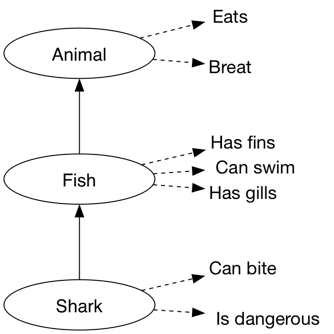
\includegraphics[width=0.60\textwidth]{MemoryStructure.png}
        \caption{A hypothetical memory structure, from \protect \citet{Collins1969}}
        \label{MemoryStructure}
    \end{center}
\end{figure}


\section{Lexitags}
\label{Lexitags}
\citet{Veres2011} marks one of the differences between the Web 2.0, or the social web and the semantic web as the
fact that the social web is based on giving users the ability to create free form, unstructured data or content.
The semantic web on the other hand is based on having a structure that allows for automatic machine processing of the content.
The advantage of the social web is that it provides a very low threshold for content providers,
but the lack of structure can provide long term difficulties since it can become hard to retrieve older content.
The semantic web on the other hand has a higher threshold,
but the structure makes retrieving the correct content easier,
since machines can reason about the content and be made responsible for finding the correct content.
The goal then would be to create a system that feels like a social system at input time,
but which creates structured markup which can be searched like a semantic system at retrieval time.

The lexitags system is developed to work with tags,
simple user provided strings containing one or a few words that are tied to the object of interest.
Analysis of tags by \citet{Tonkin2006} from delicious\footnote{\url{https://delicious.com}} and Flickr\footnote{\url{http://www.flickr.com}},
two websites that are focused on user generated content and tags,
showed that a large amount of the tags were "sloppy".
Sloppy tags could mean that the tags were misspelled,
that users had made compounded words my merging several words into one tag
or that they added non-alphanumeric characters.

One challenge tied to lexitags is mapping these types of tags,
which might not correspond to a English word, into a known vocabulary.
The vocabularies used by lexitags are WordNet and DBPedia.
Since WordNet mainly contains dictionary words,
DBPedia was chosen to complement it to cover things like names, places, or compound terms.
Lexitags solves the disambiguation problem by providing the user with a list of suggested mappings for the tag provided.
The user can then pick which sens which corresponds with the meaning the user wanted to convey\citep{Veres2011}.

\section{Suggested upper merged ontology}
The suggested upper merged ontology(\nom{SUMO}{Suggested upper merged ontology}) was created based on work from the Standard Upper Ontology(\nom{SUO}{Standard Upper Ontology}),
and is one of the proposed candidates for SUO.
The work with SUO was started to fulfill the need for a large, free, public standard ontology
created by cross discipline consortium of contributors.

The idea behind a standard upper ontology is to simplify generating new knowledge and data bases
by providing high level concepts that one can use to build upon,
and which can help with interoperability with other systems.
It could also ease the burden of working with legacy databases and knowledge stores,
as one can just map them to this common ontology, and use the language of the ontology to communicate.
It can also help combine different domain specific ontologies.
By having a common set of terms, even if just a subset,
it becomes easier to integrate the different ontologies\citep{Niles2001}.

The process involved in creating SUMO consisted of several steps.
To start with it was necessary to identify high lever ontologies which where not hampered by licensing issues.
As the name can imply, the basis of SUMO was to merge these ontologies together into one unified ontology,
using the upper concepts of these ontologies.
The upper levels are shown in figure \ref{SUMOUpper}( page \pageref{SUMOUpper}).
Physical describes all those things that have some position in time and space, things like atoms, dogs and galaxies.
The other main category, Abstract, covers those things that do not have some physical extension, like numbers,
justice, and song.
In addition to these types there is a unifying top level type called entity, which encompasses all things physical and abstract.

Before the merge could start, the different ontologies were translated into the same knowledge representation format,
to make sure they conformed to the same syntax\citep{Niles2001}.
SUMO is written in the SUO knowledge interchange format,
but is also translated to the web ontology language(\nom{OWL}{Web Ontology Language})\citep{Benzmuller2012}.
Then the ontologies which contained the highest level concepts were merged by unifying those concepts that were equal,
and positioning the other concepts in relation to them.
This upmost level was then used as a basis for aligning the other lower level ontologies\citep{Niles2001}.


Merging the lower level terms fell into four general cases.
In the simplest case the term didn't correspond to terms in the other ontologies,
but was useful and suitable, and didn't break with any of the philosophical decisions made.

Other terms were found to be unsuitable for SUMO.
Since SUMO was supposed to be a top level ontology terms that were to narrow,
or which had little practical use were discarded.

In other cases a term would refere to the same meaning as some other term in the ontology.
In these cases where it was only the term chosen to convey the meaning that differed one can map both term to the same
term in the final ontology.
In the last case the terms has overlapping meaning.
In these cases one either kept both the terms, or picked which one to use in the merged ontology.

\begin{figure}[h]
    \begin{center}
        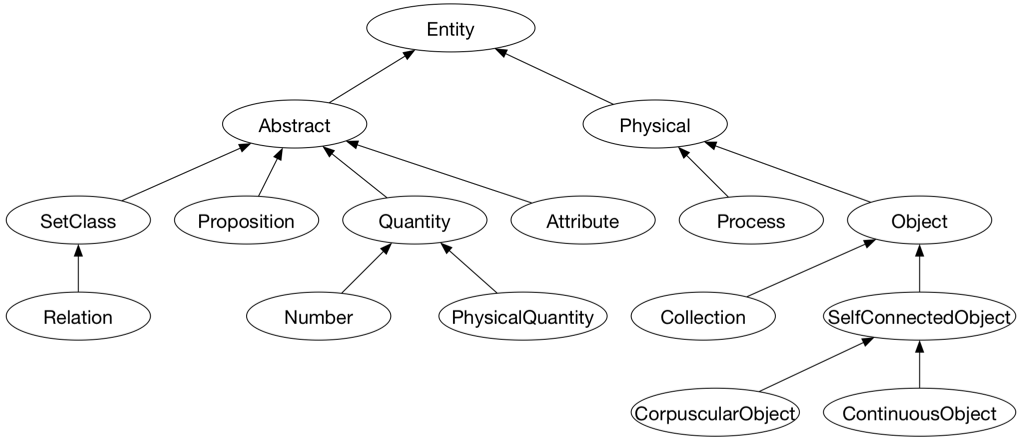
\includegraphics[width=0.80\textwidth]{SUMOUpper.png}
        \caption{The upper levels of SUMO. From \protect \citet{Niles2001}}
        \label{SUMOUpper}
    \end{center}
\end{figure}
\section{Schema.org}
Schema.org\footnote{\url{http://schema.org}} is a joint venture by Google, Yahoo, and Bing,
with the expressed goal of creating richer search results by getting content creators add meta data to their pages.
The enrichment the meta data is supposed to provide is mainly by providing information for rich snippets\citep{Guha2011}.
Rich snippets are small pieces of HTML which in some way can add information to a search result,
showing the number of stars a product got in a review, a picture of the author, some multimedia content etc\citep{Mayer2009}.
Schema.org is tied closely to the microdata format\footnote{\url{http://dev.w3.org/html5/md-LC/}},
but does at the moment still allow RDFa.

Schema.org is not a general or upper level, or a domain specific ontology,
but can be regarded as a middle level ontology.
That is to say that it does not try to be neither an all encompassing ontology,
nor an ontology which covers everything within a domain.
The role as a midlevel ontology involves covering the most common use cases without having the entire hierarchy modeled.
The top levels of schema.org are:
\begin{itemize}
	\item Thing
	\begin{itemize}
		\item Class
		\item CreativeWork
		\item Event
		\item Intangible
		\item MedicalEntity
		\item Organization
		\item Person
		\item Place
		\item Product
		\item Property
	\end{itemize}
\end{itemize}
Inspecting the ontology shows that it is clearly geared toward search engine and commercial usage,
both in the concepts that are selected, and in the hierarchal structure of the ontology\citep{Ronallo2012}.

If schema.org does not contain the term needed they suggest extending the scheme by adding sub-types or sub-properties.
The mechanism they provide for extending the vocabulary is string concatenation.
Schema.org defines person using the following URL:
\begin{verbatim}
	http://schema.org/Person
\end{verbatim}
If you need to say that this person is a minister you would then extend Person by adding Minister at the end:
\begin{verbatim}
	http://schema.org/Person/Minister
\end{verbatim}
The intention is to have the extension mechanism working in a way that will give search engines some information,
even when they come across unknown terms.
It is also intended as a way to let the ontology grow organically,
as terms which become common can be included in the schema.

This extension mechanism does however not conform with the microdata specification as \citet{Tennison2011} explains.
The specification says that URIs should be opaque identifiers,
and that one should not infere meaning through string parsing.
The mechanism also comes into difficulties when it comes to disambiguation.
It is impossible to infere from the URI it self if Person/Minister referes to a clergyman, or to a minister of state.
This problem would also persist when incorporating the term in the schema,
and might make markup that used to be correct say something that was unintended.


\section{DBPedia}
DBPedia is an ontology project based on data from Wikipedia\footnote{\url{http://www.wikipedia.org}}.
Wikipedia is a successful open collaborative information project,
with about 4.2 million articles in english and 30 million all together
\footnote{As of 2013-04-16: \url{http://en.wikipedia.org/wiki/Wikipedia:Size_of_Wikipedia}}.
The justification for the ontology is similar to the criticism mentioned by \citet{Shirky2007}
that it's difficult to know how a schema or ontology is going to be used before it's released on the web.
Instead of starting with an ontology then the work with DBPedia examine how one can extract unstructured data
from Wikipedia and transform it into a machine readable ontology.
The main contributions of the project has been\citep{Auer2007}:

\begin{itemize}
	\item Developing a framework for extracting information from Wikipedia to RDF
	\item Linking the items in the dataset to other ontologies
	\item Exposing the RDF dataset to the public
	\item Developing APIs for accessing the dataset
\end{itemize}

The extraction process is described in \citet{Auer2007a}.
DBPedia extracts information from templates on the Wikipedia pages.
The algorithm used looks through templates which have a high probability of containing structured information.
These templates are parsed looking for pairs of attributes and values.
The attributes correspond to predicates, and the values to objects of RDF statements.
The subject of the statements would be the topic of the page it self,
and it's given a unique URI in the DBPedia namespace by using it's Wikipedia URL.
There is also some post processing of the results to enhance the data further.
If the object of the statement is another Wikipedia resource,
the same process that exists for the subject is used to find the targets URL and link it to that.
In the cases where the object is a literal of a known type, then the data type information is added.

DBPedia is not a static ontology and in continuously being updated with data from Wikipedia,
making sure it's up to date with the newest terms and information.
